% $Header: /cvsroot/latex-beamer/latex-beamer/solutions/generic-talks/generic-ornate-15min-45min.en.tex,v 1.5 2007/01/28 20:48:23 tantau Exp $

\documentclass{beamer}

\usepackage{caption}
\captionsetup{labelformat=empty,labelsep=none,font=scriptsize}
\setlength{\abovecaptionskip}{0pt}

\usepackage{color}
%% These definitions are based on darkred at
%% http://www.december.com/html/spec/colorcmyk.html
\definecolor{darkred}{cmyk}{0, 1, 1, 0.45}
\newcommand{\jul}{\textcolor{darkred}}
\newcommand{\jan}{\textcolor{blue}}

% This file is a solution template for:

% - Giving a talk on some subject.
% - The talk is between 15min and 45min long.
% - Style is ornate.



% Copyright 2004 by Till Tantau <tantau@users.sourceforge.net>.
%
% In principle, this file can be redistributed and/or modified under
% the terms of the GNU Public License, version 2.
%
% However, this file is supposed to be a template to be modified
% for your own needs. For this reason, if you use this file as a
% template and not specifically distribute it as part of a another
% package/program, I grant the extra permission to freely copy and
% modify this file as you see fit and even to delete this copyright
% notice. 


\mode<presentation>
{
  \usetheme{Warsaw}
  % or ...

  \setbeamercovered{transparent}
  % or whatever (possibly just delete it)
}


\usepackage[english]{babel}
% or whatever

\usepackage[latin1]{inputenc}
% or whatever

\usepackage{times}
\usepackage[T1]{fontenc}
% Or whatever. Note that the encoding and the font should match. If T1
% does not look nice, try deleting the line with the fontenc.


%% \title[Short Paper Title] % (optional, use only with long paper titles)
%% {Presentation Title}
\title[]{Models combining rib and scapula samples - Rice Rivers study}
%\subtitle {Eastern CASTNET sites, May-Sep.~2001} % (optional)

%% \author[Author, Another] % (optional, use only with lots of authors)
%% {F.~Author\inst{1} \and S.~Another\inst{2}}
%% % - Use the \inst{?} command only if the authors have different
%% %   affiliation.
%% \author[Swall et al.]{Jenise Swall\inst{1}, Ana Rappold\inst{2}, and Lucas Neas\inst{2}
% - Use the \inst{?} command only if the authors have different
%   affiliation.

%% \institute[Universities of Somewhere and Elsewhere] % (optional, but mostly needed)
%% {
%%   \inst{1}%
%%   Department of Computer Science\\
%%   University of Somewhere
%%   \and
%%   \inst{2}%
%%   Department of Theoretical Philosophy\\
%%   University of Elsewhere}
%% % - Use the \inst command only if there are several affiliations.
%% % - Keep it simple, no one is interested in your street address.
 %% \institute[VCU]
 %% {
 %%   \inst{1}%
 %%   Dept.\ of Statistical Sciences and Operations Research\\
 %%   Virginia Commonwealth University
 %%   \and
 %%   \inst{2}%
 %%   National Health and Environmental Effects Research Laboratory\\
 %%   U.S.~Environmental Protection Agency
 %% }

%% \date[Short Occasion] % (optional)
%% {Date / Occasion}
\date{July 2022}

%% \subject{Talks}
% This is only inserted into the PDF information catalog. Can be left
% out. 



% If you have a file called "university-logo-filename.xxx", where xxx
% is a graphic format that can be processed by latex or pdflatex,
% resp., then you can add a logo as follows:

% \pgfdeclareimage[height=0.5cm]{university-logo}{university-logo-filename}
% \logo{\pgfuseimage{university-logo}}



% Delete this, if you do not want the table of contents to pop up at
% the beginning of each subsection:
% \AtBeginSection[]
% {
%  \begin{frame}<beamer>{Outline}
%    \tableofcontents[currentsection,currentsubsection]
%  \end{frame}
% }


% If you wish to uncover everything in a step-wise fashion, uncomment
% the following command: 

%\beamerdefaultoverlayspecification{<+->}

\useoutertheme{infolines}

\begin{document}

\begin{frame}
   \titlepage
\end{frame}

%% \begin{frame}{Outline}
%%  \tableofcontents
  % You might wish to add the option [pausesections]
%% \end{frame}


% Since this a solution template for a generic talk, very little can
% be said about how it should be structured. However, the talk length
% of between 15min and 45min and the theme suggest that you stick to
% the following rules:  

% - Exactly two or three sections (other than the summary).
% - At *most* three subsections per section.
% - Talk about 30s to 2min per frame. So there should be between about
%   15 and 30 frames, all told.


%% %%%%%%%%%%%%%%%%%%%%%%%%%%%%%%%%%%%%%%%%%%%%%%%%%%%%%%%%%%



%% %%%%%%%%%%%%%%%%%%%%%%%%%%%%%%%%%%%%%%%%%%%%%%%%%%%%%%%%%%
\section{Preliminaries}

\begin{frame}{Combining rib and scapula}

  \begin{itemize}
    \item I re-ran the random forest models using ribs and scapula samples combined.
    \item The models don't distinguish between ribs and scapula, so neither type
   is given more weight than the other.
    \item In general, we expect improved overall model performance due to the
    larger sample sizes obtained by combining ribs and scapulae samples.  This
    is particularly relevant for the models using swabs, since the sample sizes
    are smaller than for the bone data.
    \item However, if there are notable differences in the rib and scapula
    samples, this could adversely affect model fit and interpretation.
  \end{itemize}

\end{frame}



\begin{frame}{Choosing taxa to include}
  
  \begin{itemize}
    \item In our previous separate analyses for ribs and scapulae, we have
    required that a taxon must have a prevalence of at least 1\%  in at least 2
    samples in order to be included in the analysis.
    \item When doing the analysis using combined rib and scapula samples, we
    require that the taxa must have met this standard for \textbf{both} ribs and
    scapulae to be included.  This means that the number of taxa considered in
    the model is smaller than the numbers used in the individual rib and scapula
    models.
  \end{itemize}

\end{frame}
%% %%%%%%%%%%%%%%%%%%%%%%%%%%%%%%%%%%%%%%%%%%%%%%%%%%%%%%%%%%



%% %%%%%%%%%%%%%%%%%%%%%%%%%%%%%%%%%%%%%%%%%%%%%%%%%%%%%%%%%%
\section{Using swabs}


% %%%%%%%%%%%%%%%%%%%%%%%%%%%%%%%%%%%
\subsection{Omiting baseline observations (ADD 0)}

\begin{frame}{Random forest model combining rib and scapula samples (omitting ADD 0)}

  \begin{tabular}{lrrrr}
    Type & \# samples & \# taxa & RMSE & Expl.\ variation\\ \hline
    Ribs & 15 & 49 & 642.7 &      73.1\% \\
    Scapulae & 14 & 53 & 800.9 &  56.6\% \\
    Combined & 29 & 38 & 621.1 &  74.4\%
  \end{tabular}
  
  \vspace{0.1in}

\end{frame}


\begin{frame}{Pred.\ vs. actual ADD for swabs (without baseline obs.)}

  \begin{center}
    \begin{figure}
      \includegraphics[height=3.1in]
        {w_swabs/bacteria/use_families/rr_combined_family_no_baseline_predicted_vs_actual_ADD}
    \end{figure}
  \end{center}

\end{frame}



\begin{frame}{Influential taxa for swabs (omitting ADD 0)}

  \begin{center}
    \begin{figure}
      \includegraphics[height=2.85in]
        {w_swabs/bacteria/use_families/rr_combined_family_no_baseline_6panels}
    \end{figure}
  \end{center}

\end{frame}


\begin{frame}{Influential taxa are different}
  
  \begin{itemize}
    \item The influential taxa are different for the analyses using ribs only,
    scapulae only, and combined ribs and scapulae.
    \item This is partly because, to be included in the combined rib/scapula
    model, a taxon must have a prevalence of at least 1\% in at least 2 rib
    samples \textbf{and} at least 2 swab samples.
    \begin{itemize}
      \item The following influential taxa in the rib model were not included in
    the combined rib/scapula model:\\
    Haliangiaceae and Rhodospirillaceae
    \item The following influential taxa in the scapula model were not included
    in the combined rib/scapula model:\\
    Methylocystaceae and Tissierellaceae
    \end{itemize}
    \item The following taxa were in the "top 10" influential taxa for all
    three models:\\
    Enterobacteriaceae and Methylococcaceae
  \end{itemize}

\end{frame}
% %%%%%%%%%%%%%%%%%%%%%%%%%%%%%%%%%%%



% %%%%%%%%%%%%%%%%%%%%%%%%%%%%%%%%%%%
\subsection{Including baseline observations (with ADD 0)}

\begin{frame}{Random forest model combining rib and scapula samples (using ADD 0)}

  \begin{tabular}{lrrrr}
    Type & \# samples & \# taxa & RMSE & Expl.\ variation\\ \hline
    Ribs & 18 & 49 & 607.8 & 81.8\% \\
    Scapulae & 17 & 53 & 681.4 & 76.6\% \\
    Combined & 35 & 38 & 580.2 & 83.2\%
  \end{tabular}
  
  \vspace{0.1in}

\end{frame}


\begin{frame}{Pred.\ vs. actual ADD for swabs (with baseline obs.)}

  \begin{center}
    \begin{figure}
      \includegraphics[height=3.1in]
        {w_swabs/bacteria/use_families/rr_combined_family_w_baseline_predicted_vs_actual_ADD}
    \end{figure}
  \end{center}

\end{frame}



\begin{frame}{Influential taxa for swabs (with ADD 0)}

  \begin{center}
    \begin{figure}
      \includegraphics[height=2.85in]
        {w_swabs/bacteria/use_families/rr_combined_family_w_baseline_6panels}
    \end{figure}
  \end{center}

\end{frame}


\begin{frame}{Comments about influential taxa}

  \begin{itemize}
    \item Methylococcaceae is influential in each of the analyses.
    \item The following influential taxa in the rib model were not included in
    the combined rib/scapula model:\\
    Rhodospirillaceae and Desulfobacteraceae
    \item The following influential taxon in the scapula model was not included
    in the combined rib/scapula model:\\
    Methylocystaceae
    \item The following taxa were in the "top 10" influential taxa for all
    three models:\\
    Methylococcaceae, Crenotrichaceae, Holophagaceae
  \end{itemize}

\end{frame}
%% %%%%%%%%%%%%%%%%%%%%%%%%%%%%%%%%%%%%%%%%%%%%%%%%%%%%%%%%%%





%% %%%%%%%%%%%%%%%%%%%%%%%%%%%%%%%%%%%%%%%%%%%%%%%%%%%%%%%%%%
\section{Using bones}


% %%%%%%%%%%%%%%%%%%%%%%%%%%%%%%%%%%%
\subsection{Omiting baseline observations (ADD 0)}

\begin{frame}{Random forest model combining rib and scapula samples (omitting ADD 0)}

  \begin{tabular}{lrrrr}
    Type & \# samples & \# taxa & RMSE & Expl.\ variation\\ \hline
    Ribs & 81 & 41 & 476.6 & 93.2\% \\
    Scapulae & 110 & 55 & 500.7 &  92.8\% \\
    Combined & 191 & 38 & 564.2 & 90.7\%
  \end{tabular}
  
  \vspace{0.2in}

  \footnotesize{
    \noindent It's interesting that the combined model doesn't perform as well
    here as the other models.
  }

\end{frame}



\begin{frame}{Differences in taxa prevalence between ribs and scapulae (omitting ADD 0)}

  \begin{center}
    \begin{figure}
      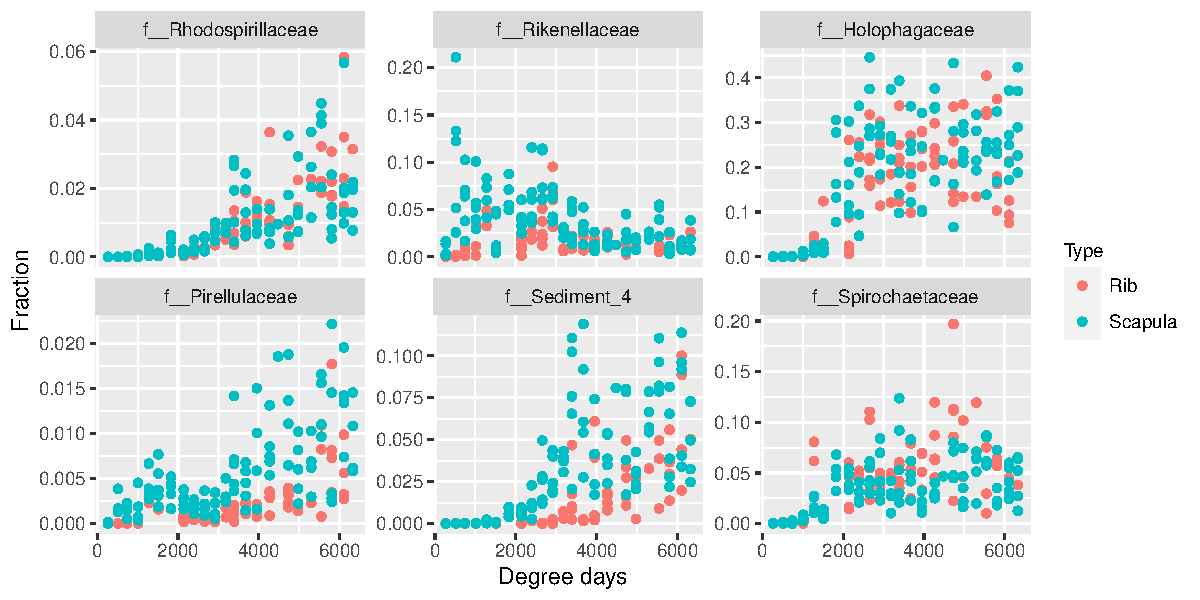
\includegraphics[height=2.0in]
        {w_bones/bacteria/use_families/both_ribs_scapulae/no_baseline/infl_combined_bone_no_baseline_family_scatter}
    \end{figure}
  \end{center}

  \footnotesize{
    \noindent For some of the taxa, it looks like their prevalence
    for rib and scapula samples may be substantially different.  This may
    "confuse" the combined model.  In the next slide, you can see that we seem
    to be overpredicting more often for the scapulae.
    }

\end{frame}



\begin{frame}{Pred.\ vs. actual ADD for bones (without baseline obs.)}

  \begin{center}
    \begin{figure}
      \includegraphics[height=3.1in]
        {w_bones/bacteria/use_families/rr_combined_family_no_baseline_predicted_vs_actual_ADD}
    \end{figure}
  \end{center}

\end{frame}



\begin{frame}{Influential taxa for bones (omitting ADD 0)}

  \begin{center}
    \begin{figure}
      \includegraphics[height=2.85in]
        {w_bones/bacteria/use_families/rr_combined_family_no_baseline_6panels}
    \end{figure}
  \end{center}

\end{frame}


\begin{frame}{Comments about influential taxa (omitting ADD 0)}
  
  \begin{itemize}
    \item The influential taxa are more similar in these analyses than they were
    for the swabs.
    \item The following influential taxa in the scapula model were not included
    in the combined rib/scapula model:\\
    Dethiosulfovibrionaceae, Syntrophaceae, Syntrophobacteraceae
    \item The following taxa were in the "top 10" influential taxa for all
    three models:\\
    Rhodospirillaceae and Sediment\_4 \quad (Is the latter actually a taxon?) 
  \end{itemize}

\end{frame}
% %%%%%%%%%%%%%%%%%%%%%%%%%%%%%%%%%%%




% %%%%%%%%%%%%%%%%%%%%%%%%%%%%%%%%%%%
\subsection{Including baseline observations (with ADD 0)}

\begin{frame}{Random forest model combining rib and scapula samples (using ADD 0)}

  \begin{tabular}{lrrrr}
    Type & \# samples & \# taxa & RMSE & Expl.\ variation\\ \hline
    Ribs & 84 & 41 & 473.3 & 93.7\% \\
    Scapulae & 115 & 55 & 498.5 & 93.4\% \\
    Combined & 199 & 38 & 560.9 & 91.4\%
  \end{tabular}
  
  \vspace{0.2in}

  \footnotesize{
    \noindent Again, we see that the combined model doesn't perform quite as
    well as the other two.
  }


\end{frame}


\begin{frame}{Differences in taxa prevalence between ribs and scapulae (using ADD 0)}

  \begin{center}
    \begin{figure}
      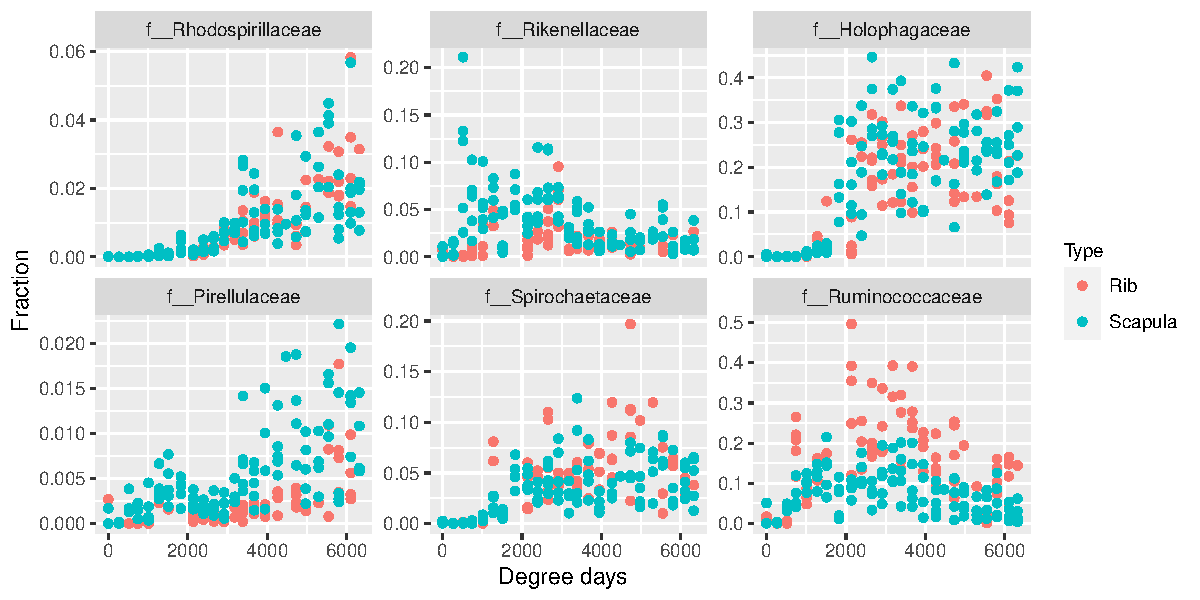
\includegraphics[height=2.0in]
        {w_bones/bacteria/use_families/both_ribs_scapulae/w_baseline/infl_combined_bone_w_baseline_family_scatter}
    \end{figure}
  \end{center}

  \footnotesize{
    \noindent Again, it looks like the prevalences of some taxa may differ for
    rib and scapula samples.
    }

\end{frame}



\begin{frame}{Pred.\ vs. actual ADD for bones (with baseline obs.)}

  \begin{center}
    \begin{figure}
      \includegraphics[height=3.1in]
        {w_bones/bacteria/use_families/rr_combined_family_w_baseline_predicted_vs_actual_ADD}
    \end{figure}
  \end{center}

\end{frame}



\begin{frame}{Influential taxa for bones (with ADD 0)}

  \begin{center}
    \begin{figure}
      \includegraphics[height=2.85in]
        {w_bones/bacteria/use_families/rr_combined_family_w_baseline_6panels}
    \end{figure}
  \end{center}

\end{frame}


\begin{frame}{Comments about influential taxa (with ADD 0)}
  
  \begin{itemize}
    \item We have more bone samples, so it doesn't make as much difference
    whether we include ADD 0, compared to the results of the swab analyses.
    \item The following influential taxa in the scapula model were not included
    in the combined rib/scapula model:\\
    Dethiosulfovibrionaceae, Syntrophaceae, Syntrophobacteraceae
    \item The following taxa were in the "top 10" influential taxa for all
    three models:\\
    Rhodospirillaceae, Ruminococcaceae, Sediment\_4 \quad (Again, is the latter actually a taxon?) 
  \end{itemize}

\end{frame}


\end{document}
